\documentclass[tikz,border=3pt]{standalone}
\usepackage{lmodern}
\usepackage{xcolor}
\usetikzlibrary{arrows.meta}


\begin{document}
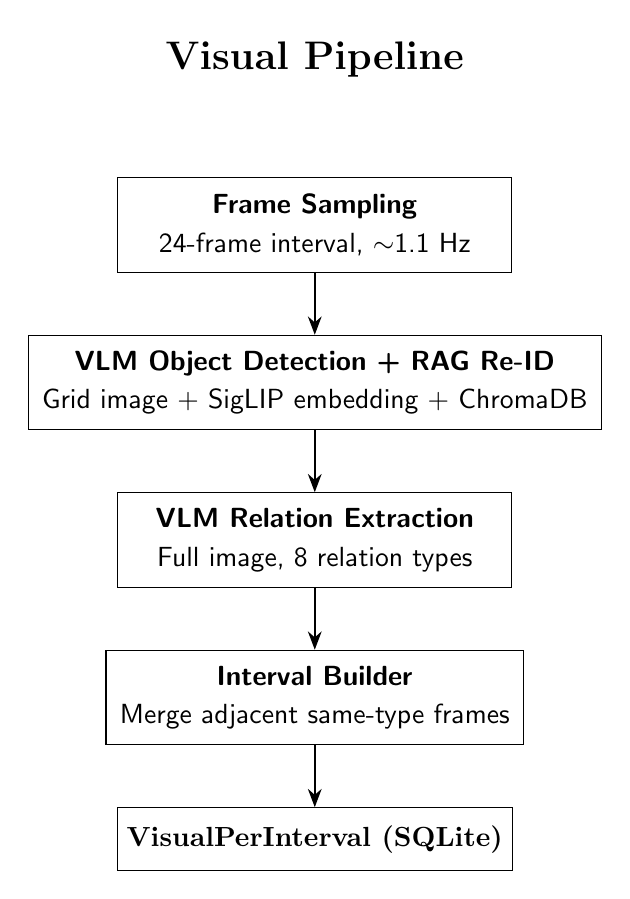
\begin{tikzpicture}[
  every node/.style={font=\sffamily},
  box/.style={draw=black, align=center, inner sep=5pt, minimum width=5cm, minimum height=1.2cm},
  arrow/.style={-Stealth, thick},
]

\draw[white] (-0.3,-0.5) rectangle (5.6,8.3);

\node[font=\Large\bfseries] at (2.5,7.9) {Visual Pipeline};

\node[box,fill=white] (s1) at (2.5,5.8) {
    \textbf{Frame Sampling}\\[2pt]
    24-frame interval, ${\sim}$1.1 Hz
};

\node[box,fill=white] (s2) at (2.5,3.8) {
    \textbf{VLM Object Detection + RAG Re-ID}\\[2pt]
    Grid image + SigLIP embedding + ChromaDB
};

\node[box,fill=white] (s3) at (2.5,1.8) {
    \textbf{VLM Relation Extraction}\\[2pt]
    Full image, 8 relation types
};

\node[box,fill=white] (s4) at (2.5,-0.2) {
    \textbf{Interval Builder}\\[2pt]
    Merge adjacent same-type frames
};

\node[draw=black, fill=white, font=\normalsize\bfseries, align=center, minimum width=5cm, minimum height=0.8cm] (out) at (2.5,-2.0) {VisualPerInterval (SQLite)};

\draw[arrow] (s1.south) -- (s2.north);
\draw[arrow] (s2.south) -- (s3.north);
\draw[arrow] (s3.south) -- (s4.north);
\draw[arrow] (s4.south) -- (out.north);

\end{tikzpicture}
\end{document}
